\chapter{Análise Exploratória de Dados}\label{eda}

A análise exploratória de dados, mais conhecida como \textit{Exploratory Data
Analysis} (\textit{EDA}), são procedimentos para a análise de dados, técnicas
para a interpretação dos resultados de tais procedimentos, formas de
planejamento da coleta de dados para fazer a sua análise mais fácil, mais precisa
e mais acurada, e todo o maquinário e resultados estatísticos que se aplicam aos
dados \cite{tukey:1961}. A análise exploratória de dados traz uma variedade de
técnicas para, por exemplo, encontrar características escondidas dos dados,
extrair variáveis importantes e detectar anomalias e \textit{outliers}, sendo
\textit{outlier} um número que é muito maior ou menor que o resto dos números em
uma dada série de números \cite{hawkins80}. Segundo \citeonline{wasiak:2012},
o principal objetivo da abordagem de análise exploratória de dados é adiar as
premissas habituais sobre que tipo de modelo os dados seguem com uma abordagem
mais direta de permitir que os dados revelem a sua estrutura e o modelo.

Para apresentar a análise de dados exploratória foi feita uma rápida comparação
com outros métodos de análise de dados, sendo eles as análises clássica e
bayesiana. A Figura \ref{fig:analysis_comparacao} apresenta um diagrama de
sequência de atividades dos métodos de análises de dados que aqui serão
comparados.

\begin{figure}[h]
  \centering
  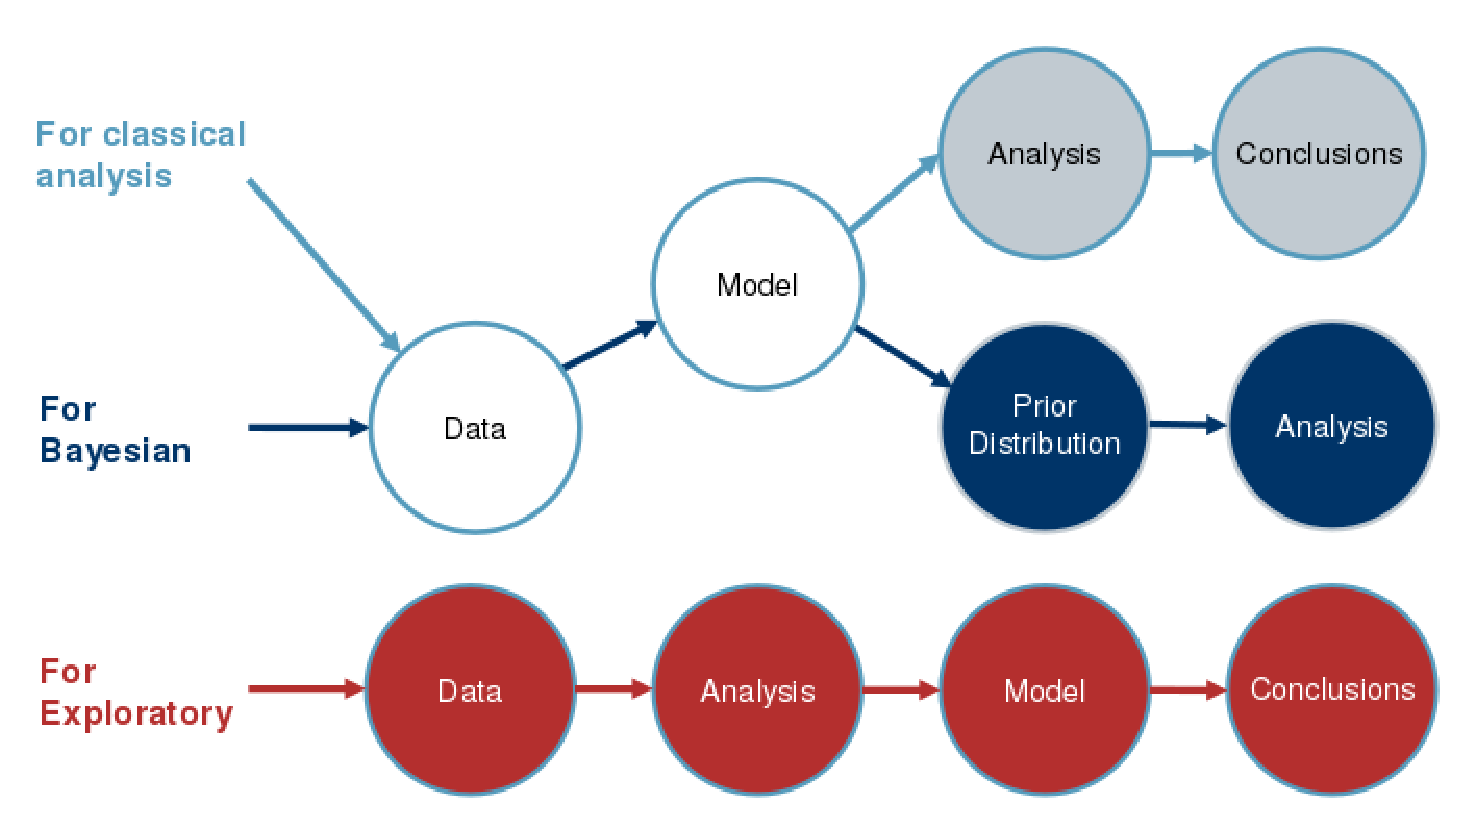
\includegraphics[width=0.8\textwidth]
      {figuras/analysis_comparacao}
      \caption{Sequência de atividades dos métodos de
      análise \cite{wasiak:2012}}
  \label{fig:analysis_comparacao}
\end{figure}

Como pode-se ver na sequência de atividades apresentadas na Figura
\ref{fig:analysis_comparacao}, os métodos clássico e bayesiano tendem a definir
um modelo para os dados antes de realizar qualquer tipo de análise, a análise é
feita apenas após a definição do modelo, esse tipo de abordagem pode levar a
elaboração de modelos não satisfatórios e isso só será identificado após a
análise desse modelo construído. Esse tipo de erro torna o processo de definição
de um modelos bastante custoso, onde deverá ser realizado o processo de análise
várias vezes até atingir um resultado satisfatório. Já a abordagem de análise
exploratória de dados, como foi dito anteriormente no início do capítulo, visa a
exploração dos dados antes da definição do modelo, deixando os dados
apresentarem as suas estruturas e qual possível modelo melhor se adequa àqueles
dados.

\section{Análise dos dados}

No início da análise exploratório de qualquer tipo de dados é importante
entendê-los, verificar possíveis correlações entre os mesmos e se necessário
derivar novas características dos dados que auxiliem na exploração dos mesmos.

Para isso pode-se utilizar de algumas técnicas como o coeficiente de correlação
de Pearson, sendo essa uma técnica da estatística descritiva, que visa medir a
direção e grau com que duas variáveis, de tipo quantitativo, se associam
linearmente \cite{rossman:1996}. Uma técnica que pode-se utilizar do método de
correlação de Pearson é a contrução de uma matriz de correlação, onde todos os
dados são confrontados para tentar encontrar algum tipo de dependência linear
entre os mesmos. 

Com essas informações em mãos pode-se realizar por exemplo uma engenharia de
características, sendo engenharia de características a utilização de
características existentes para gerar novas características que aumentem o valor
da base de dados original, utilizando conhecimento dos dados ou do domínio em
questão \cite{brink:2014}. Além disso, pode-se remover características
dispensáveis do conjunto de dados, que possam ser redundantes com outras
características por exemplo. Em suma, engenharia de característica é o processo
de transformar dados nunca trabalhados em características que melhor representam
o problema atacado para o modelo preditivo, resultando em uma precisão de modelo
melhorada nos dados escondidos \cite{brownlee:2014}.

\section{Técnica de Visualização dos Dados}\label{4-plot}

Para a realização dessa análise exploratória dos dados antes da definição de um
modelo são utilizados vários tipos de técnicas gráficas, tornando-as muito
importantes dentro do processo. Uma técnica simples e que reuni um grupo de
gráficos para trazer uma visão geral sobre os dados trabalhados é a
\textit{4-Plot} trazido pelo
\textit{Handbook}\footnote{\url{http://www.itl.nist.gov/div898/handbook/eda/section3/eda3332.htm}}
sobre análise exploratória desenvolvido pelo \textit{NIST} (\textit{National
Institute of Standards and Technology}), essa técnica nos possibilita entender
desde se a distribuição dos dados segue uma distribuição normal até a sua
aleatoriedade. Identificar esses tipos de características revelam informações
importantes para a definição de um modelo que satisfaça determinado conjunto de
dados, ou pelo menos elimar opção indesejadas. Os tipos de representação gráfica
apresentado por essa abordagem \textit{4-Plot} são histograma, \textit{Q-Q
Plot}, \textit{Run Sequence} e \textit{Lag Plot}, como pode ser visto na Figura
\ref{fig:4-plot}, sendo os gráficos superior esquerdo o \textit{Run Sequence},
superior diretor o \textit{Lag Plot}, inferior esquerdo o histograma e o
inferior esquerdo o \textit{Q-Q Plot}.

\begin{figure}[h]
  \centering
  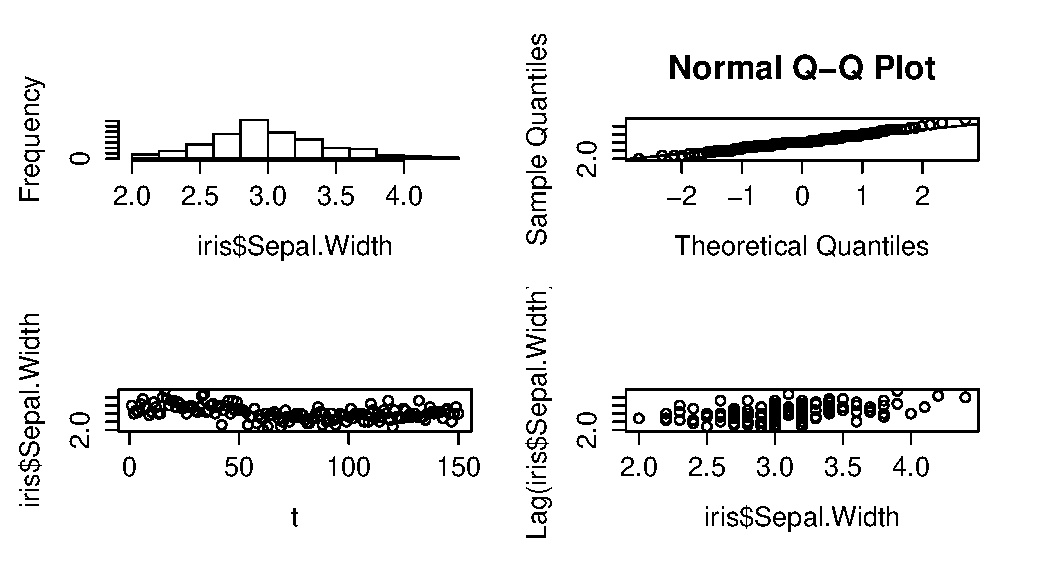
\includegraphics[width=1.0\textwidth]
      {figuras/4-plot}
      \caption{Exemplo \textit{4-Plot}}
  \label{fig:4-plot}
\end{figure}

Através do histograma consegue-se identificar a distribuição dos dados, a partir
dele juntamente com o \textit{Q-Q Plot} pode-se identificar se a distribuição
dos dados segue uma distribuição normal ou não, sendo o \textit{Q-Q Plot} um
gráfico que confronta os quantis de uma distribuição normal e os quantis da
distribuição dos dados em questão. se ambos forem similares, tendem a traçar uma
reta diagonal. O gráfico \textit{Run Sequence} visa apresentar uma forma de
verificar se a variância da distribuição dos dados é constante ou não,
apresentando possíveis deslocamentos, para isso é plotado um índice incremental
pelo valor variável dependente. Já o gráfico \textit{Lag Plot} tenta mostrar a
aleatoriedade dos dados, onde são plotados seguindo a ordem do conjunto de dados
o seu valor diretamente antecessor pelo valor atual, dessa forma, se os dados da
distriubição forem realmente aleatórios os pontos deverem ficar espalhados pelo
gráfico, caso siga algum tipo de padrão, a hipótese é negada.


\section{Identificação de \textit{Outliers}}\label{outliers}

Um passo importante para atingir um modelo que se adeque bem aos seus dados é a
identificação e remoção dos possíveis \textit{outliers}. Um método bastante
simples para identificação de \textit{outliers} apresentado por
\citeonline{tukey:1977} é utilizar o gráfico \textit{boxplot}. Como pode ser
visto na Figura \ref{fig:boxplot}, o gráfico possui uma linha central da caixa
representanado a mediana do conjunto de dados, a superior o 3º quartil e a inferior
o 1º quartil, a diferença entre os quartis é chamada \textit{IQR}
(\textit{Interquantile Range}). A técnica trazido por \citeonline{tukey:1977}
consiste em limitar os valores válidos, ou seja, não \textit{outliers}, até
150\% do valor do respectivo \textit{IQR} a mais e a menos dos quartis que
limitam a caixa, valores que extrapolem isso são considerados \textit{outliers}.

\begin{figure}[h]
  \centering
  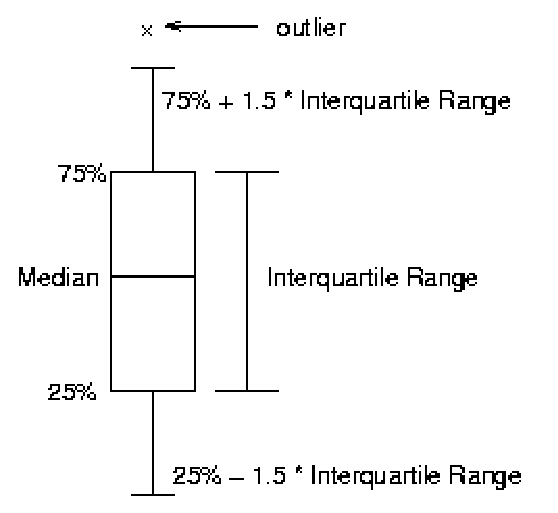
\includegraphics[width=0.5\textwidth]
      {figuras/boxplot}
      \caption{Explicação sobre identificação de \textit{outliers} com
      \textit{boxplot}}
  \label{fig:boxplot}
\end{figure}

\section{Definição de Modelos}\label{defmodels}

Após o entendimento de algumas características inerentes aos dados e
identificação e remoção de \textit{outliers}, necessita-se definir um modelos
que se adapte ao conjunto de dados com uma certa flexibilidade, ou seja,
evitando o \textit{overfitting}, que seria o modelo se justar demais aos dados
ao ponte do mesmo não conseguir extrapolar para outros valores. Para a definição
de um modelo pode-se utilizar métodos paramétricos ou não paramétricos
dependendo das informações que se tem em mão e que foram extraídas do conjunto
de dados. Um modelo não paramétrico bastante robusto e simples de utilizar é o
\textit{Locally Weighted Regression} (muito conhecido como \textit{LOESS})
apresentado por \citeonline{cleveland:1988}, esse método possui três objetivos
principais: exploração dos dados, diagnosticar métodos não paramétricos e prover
uma superfície suave utilizando um regressão não paramétrica. Com isso, esse
método pode nortear a definição de um possível modelo paramétrico. Basicamente
esse modelo realiza várias pequenas regressões no conjunto de dados, conhecido
como janelamento, definindo pesos para cada uma dos pontos vizinhos dependendo da
função que se utiliza, em geral, se utiliza uma função tricúbica
\cite{cleveland:1988}. Essas várias regressões acabam resultando em um modelo
que apresenta uma curva de predição bastante suave, sendo um ponto a se
considerar o fato do método ser ``caixa preta'', não permitindo a obtenção de
uma fórmula matemática que represente o modelo. Outra forma de se definir um
modelo é a partir da utilização de um método paramétrico, sendo a regressão
polinomial um dos mais conhecidos. A regressão polinomial implementada por boa
parte das ferramentas geralmente é feita através do método dos mínimos
quadrados, que visa diminuir o erro gerado pelo modelo ao máximo.

\section{Validação de Modelos}\label{valmodels}

Para a validação de modelos construídos pode-se utilizar várias técnicas, aqui
serão apresentadas a \textit{ANOVA} e validação cruzada \textit{K-Fold}. A
Análise de Variância, mais conhecida como \textit{ANOVA}, visa análisar a
variância entre o resultado obtido pelo modelo e o valor real, também sendo
utilizada para comparação de modelos, onde é possível verificar a variância
quando se adiciona algum elemento novo ao modelo. Para a utilização da
\textit{ANOVA} algumas suposições acerca do modelo em questão devem ser
respeitadas, como independência entre os valores ou aleatoriedade, a normalidade
dos dados e a igualdade das variâncas do conjunto de dados \cite{snedecor:1967}.
Como pode-se ver a abordagem \textit{4-Plot}, apresentada na seção \ref{4-plot},
consegue responder todas essas suposições listadas. 

Outra técnica que pode auxiliar na validação de um modelo é a técnica de
validação cruzada \textit{K-Fold}, que consiste em dividir o seu conjunto de
dados em \textit{K} grupos, onde um deles é usado para o teste do modelo e
os outros para o treinamento do mesmo, a acurácia dos resultados pode então ser
medida por meio da comparação dos resultados obtidos com os esperados
\cite{tassia:2011}. O passo-a-passo dessa técnica, segundo
\citeonline{tassia:2011}, pode ser visto a seguir:

\begin{enumerate}
  \item O conjunto de dados original é particionado aleatoriamente em k
    subconjuntos
  \item Em cada uma das \textit{K} rodadas:
    \begin{itemize}
      \item Um dos subconjuntos é reservado para testar o modelo
      \item Os demais subconjuntos são passados ao modelo como dados de treinamento
      \item Uma predição é gerada e avaliada por meio de métricas pertinentes
    \end{itemize}
  \item Ao final dos testes, os k resultados são combinados para produzir uma
    estimativa única
\end{enumerate}

Esse tipo de validação cruzada consegue nos mostrar como que o modelo se
comportaria em uma situação real de predição, onde os valores que devem ser
preditos não fazem parte do conjunto de treinamento. Como é conhecido os valores
reais desses pontos, o erro de predição do modelo pode ser calculado, usando por
exemplo o erro médio quadrático, que nada mais é do que a diferença entre o
valor estimado e o valor real dos dados, ponderados pelo número de termos
\cite{caetano:2012}, como pode ser visto na equação a seguir:

\begin{align*}
  EMQ = \sum (y - \hat{y}) / n
\end{align*}

Na equação acima, o valor de \textit{y} representa o valor estimado,
\textit{y} chapéu o valor real e \textit{n} o número total de elementos dentro do
conjunto de dados. Outro métrica que também pode ser utilizada é o erro residual
padrão que nada mais é do que o desvio padão do erro residual, que é a diferença
entre o valor real e o predito.



Neste capítulo foram apresentados de forma objetiva apenas as técnica e
conceitos utilizados neste trabalho, não explorando os diferentes métodos e tipos de
abordagem disponíveis, apesar desse ramo da estatística ser amplo e haver diferentes formas
de abordar um mesmo problema. Isso foi feito a fim de facilitar a leitura e
entendimento do que foi feito, seguindo o fluxo da pesquisa realizada.
